\chapter{Implementierung}
\label{ch:implementierung}

\section{Netzwerk- und Speicherstruktur der Container-Umgebung}
Die gesamte Umgebung wird durch eine \texttt{docker-compose.yml} orchestriert. Orchestrierung bedeutet die automatische Vernetzung und Verwaltung der erstellten Container, sodass diese als zusammenhängendes System funktionieren \parencite{AWS}. In der \texttt{docker-compose.yml} wird das interne Netzwerk \texttt{matomo\textunderscore network} erstellt, über welches die Container miteinander kommunizieren. Zusätzlich werden persistente Volumes definiert, um sicherzustellen, dass die Daten über Neustarts der Container hinweg erhalten bleiben. Das Volume \texttt{matomo} speichert sämtliche Konfigurationsdateien des Webanalysetools. Somit können die Matomo Einstellungen, beispielsweise für den Datenschutz persistent gespeichert werden. Die Datenbank, welche alle erfassten Trackingdaten enthält wird in dem Volume \texttt{db} gespeichert. Für die Visualisierung speichert das Volume \texttt{grafana-storage} die Konfigurationen von Grafana, sowie die erstellten Dashboards und Pannels. Das Bildungsportal wird als externes Volume \texttt{portal} aus dem Projektverzeichnis eingebunden.

\section{Reverse Proxy und Dienstweiterleitung}
Der Reverse Proxy (Nginx) wird als Zugangspunkt für die Dienste verwendet. Die Konfigurationsdatei \texttt{reverse\textunderscore proxy.conf} dient dazu, die externen Anfragen an die Dienste weiterzuleiten. Somit werden die Website, Matomo und Grafana unter separaten Pfaden erreichbar gemacht: 

\textbf{Matomo} wird über den Reverse Proxy unter \texttt{/matomo} bereitgestellt. Da das verwendete Matomo-Docker-Image \texttt{/matomo:5.2.2-fpm-alpine} keinen eigenen Webserver mitbringt, wird in der \texttt{docker-compose.yml} ein zusätzlicher Nginx-Webserver (\texttt{matomo\textunderscore web}) definiert. Dieser empfängt Anfragen vom Reverse Proxy und leitet sie über das FastCGI-Protokoll an PHP-FPM (FastCGI Process Manager) weiter, da Matomo auf PHP basiert. PHP-FPM ist ein Prozessmanager für PHP \parencite{PHPFPM}, welcher von Matomo verwendet wird. Da Nginx als Reverse Proxy keine PHP-Skripte selbst verarbeiten kann, sondern diese an eine externe Instanz übergeben muss \parencite{NginxReverseProxy}, ist dieser zusätzliche Webserver erforderlich. Dieser benötigt ebenfalls eine Konfig-Datei (\texttt{matomo.conf}), die sicherstellt, dass alle Anfragen korrekt verarbeitet und an PHP-FPM übergeben werden. Während die \texttt{reverse\textunderscore proxy.conf} externe Anfragen an \texttt{/matomo} an \texttt{matomo\textunderscore web} weiterleitet, definiert die \texttt{matomo.conf}, wie diese innerhalb des Containers verarbeitet werden. Der \texttt{matomo\textunderscore web}-Container besitzt kein öffentliches Port-Mapping und ist ausschließlich über den Reverse Proxy erreichbar.

\textbf{Grafana} wird unter \texttt{/grafana} bereitgestellt. Im Gegensatz zu Matomo benötigt Grafana keinen separaten Webserver, da es über einen integrierten Webserver verfügt. Dadurch kann Grafana direkt über den Reverse Proxy erreichbar gemacht werden.

\textbf{Die Website} wird unter \textit{evaschiffmann.de} bereitgestellt. Sie wird ebenfalls wie Matomo über einen Nginx-Webserver ausgeliefert, der ausschließlich für die Bereitstellung der Inhalte zuständig ist. Genauso wie \texttt{matomo\textunderscore web} besitzt auch dieser Webserver kein öffentliches Port-Mapping, sodass die Website nur über den Reverse Proxy aufgerufen werden kann. Dieser nimmt die Anfragen entgegen und leitet sie an den internen Nginx-Container weiter, welcher die Website ausliefert.

\begin{figure}[H]
    \centering
    \begin{minipage}{\textwidth}
        \lstinputlisting[
            caption=Docker Container zur Bereitstellung des Nginx Reverse Proxy, 
            label={lst:reverseproxy},
            language={}, 
            style=yaml
        ]{listings/reverse-proxy.yml}
    \end{minipage}
\end{figure}

Das Listing~\ref{lst:reverseproxy} zeigt die Definition des Reverse Proxy in der \texttt{docker-compose.yml}. Die einzelnen Komponenten werden anhand der Kommentare beschrieben. Um die Dienste über HTTPS verfügbar zu machen, wurde für die Testumgebung auf localhost ein selbst signiertest Zertifikat hierfür erstellt und eingebunden.

\section{Integration der Webanalyse mit Matomo}
Nachdem die Webserver aufgesetzt wurden und die \texttt{docker-compose.yml} definiert wurde, ist Matomo in der lokalen Umgebung über \textit{https://localhost/matomo} verfügbar und die Einrichtung kann erfolgen. Die Einrichtung besteht im wesentlichen aus fünf Schritten. Zunächst wird ein System Check durchgeführt, bei dem überprüft wird, ob die Serverumgebung die Anforderungen für den Betrieb von Matomo erfüllt. Hierbei wird unter anderem geprüft, ob eine kompatible PHP-Version verwendet wird oder auch ob Matomo auf die notwendigen Verzeichnisse zugreifen kann und Schreibrechte für diese besitzt. Nach dem erfolgreichen System Check kann die Datenbankverbindung eingerichtet werden und ein Hauptadministrator angelegt werden. 

\begin{figure}[H]
    \centering
    \begin{minipage}{0.49\textwidth}
        \centering
        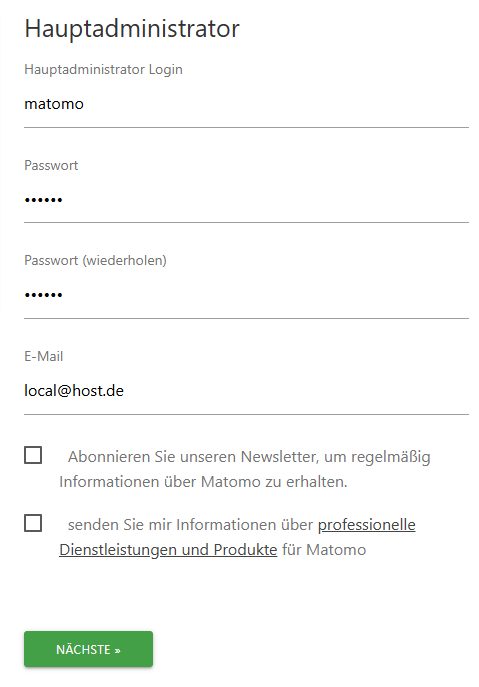
\includegraphics[width=\linewidth, keepaspectratio]{images/haupadministrator.png}
        \caption{Anlegen des Kontos für den Hauptadministrator in Matomo}
        \label{fig:hauptadministrator}
    \end{minipage}
    \hfill
    \begin{minipage}{0.49\textwidth}
        \centering
        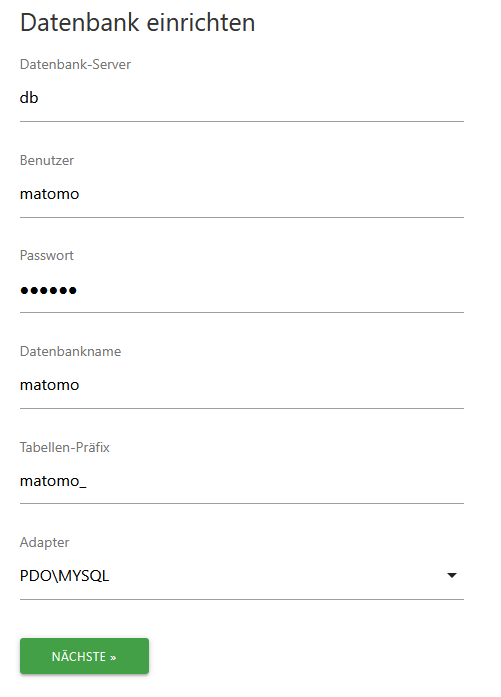
\includegraphics[width=\linewidth, keepaspectratio]{images/setup-datenbank.png}
        \caption{Einrichtung der Datenbankverbindung in Matomo}
        \label{fig:setup-datenbank}
    \end{minipage}
\end{figure}

In Abbildung~\ref{fig:hauptadministrator} ist zu sehen wie das Konto erstellt wird. In Abbildung~\ref{fig:setup-datenbank} wird gezeigt, wie die Datenbankverbindung zu MariaDB hergestellt wird. Die Zugangsdaten für den Hauptadministrator, sowie den Datenbanknutzer sind in der Datei \texttt{db.env} gespeichert. Für die Datenbank wird der Container \texttt{db} verwendet. In diesem Container wird dafür gesorgt das folgendes Skript eingebunden wird: 

\begin{figure}[H]
    \centering
    \begin{minipage}{\textwidth}
        \lstinputlisting[
            caption=SQL-Skript für die Erstellung eines Nutzer mit read-only Rechten, 
            label={lst:readonly},
            language=sql
        ]{listings/create-read-only-user.sql}
    \end{minipage}
\end{figure}

Das in Listing~\ref{lst:readonly} zu sehende Skript erstellt einen neuen Datenbanknutzer, welcher ausschließlich Leseberechtigung auf die Datenbanktabellen von Matomo besitzt. Dieser Datenbanknutzer soll später für die Anbindung an Grafana verwendet werden, um sicherzustellen, dass über Grafana keine Daten manipuliert werden können. Im vorletzten Schritt 


Datenschutzmaßnahmen:

    Anonymisierung der IP-Adressen
    Opt-out-Möglichkeit
    Erweiterung des Cookie-Consent-Banners

\section{Datenverarbeitung und Visualisierung mit Grafana}
5.3.1 Anbindung von Grafana an Matomo

    Verbindung zur MariaDB-Datenbank
    Einrichtung der Datenquelle in Grafana
    Übersicht über relevante Tabellen und deren Struktur

\section{Umsetzung der Metriken und KPIs in Grafana}


\section{Herausforderungen }